% !TEX program = pdflatex
%==================================================================
% Naskah Jurnal - disesuaikan dengan format "2024 Infomedia Template
% Format.docx" (Jurnal Infomedia: Teknik Informatika, Multimedia,
% dan Jaringan) berdasarkan isi Skripsi Muhammad Kholis.
%
% Catatan font: template asli menggunakan Book Antiqua. Karena
% dokumen ini dikompilasi dengan pdfLaTeX, font disubstitusi dengan
% Palatino (mathpazo) sebagai padanan terdekat yang tersedia.
%==================================================================
\documentclass[a4paper,10pt,onecolumn]{article}

\usepackage[indonesian,english]{babel}
\usepackage[utf8]{inputenc}
\usepackage[T1]{fontenc}
\usepackage{mathpazo} % padanan terdekat untuk Book Antiqua
\usepackage{geometry}
\geometry{a4paper, left=2.5cm, right=2.5cm, top=2.5cm, bottom=2.5cm}
\usepackage{graphicx}
\graphicspath{{../Project/gambar/}}
\usepackage{float}
\usepackage{setspace}
\usepackage{indentfirst}
\setlength\parindent{0.5cm}
\usepackage{tabularx}
\usepackage{booktabs}
\usepackage{amsmath}
\usepackage{amssymb}
\usepackage{enumitem}
\setlist{nosep}
\usepackage[font=small,labelfont=bf,justification=raggedright,singlelinecheck=false]{caption}
\usepackage[hidelinks]{hyperref}
\usepackage{fancyhdr}
\usepackage{titlesec}
\usepackage{lastpage}

% ---- Judul section: 11pt bold huruf kapital, seperti "PENDAHULUAN (11pt, Book Antiqua)"
\titleformat{\section}{\fontsize{11pt}{13pt}\bfseries}{\Roman{section}.}{0.4em}{\MakeUppercase}
\titlespacing*{\section}{0pt}{10pt}{4pt}
\titleformat{\subsection}{\fontsize{10pt}{12pt}\bfseries}{\Alph{subsection}.}{0.4em}{}
\titlespacing*{\subsection}{0pt}{6pt}{3pt}

% ---- Header/footer jurnal
\pagestyle{fancy}
\fancyhf{}
\renewcommand{\headrulewidth}{0.4pt}
\fancyhead[L]{\fontsize{8pt}{9pt}\selectfont Jurnal Infomedia : Teknik Informatika, Multimedia, dan Jaringan}
\fancyhead[R]{\fontsize{8pt}{9pt}\selectfont Volume x, Number x, Month 2026. xx-xx}
\fancyfoot[C]{\fontsize{8pt}{9pt}\selectfont \thepage}

\setstretch{1.0} % one single space

\begin{document}

%==================================================================
% KOP JURNAL
%==================================================================
\noindent
\begin{minipage}{0.68\textwidth}
    \fontsize{9pt}{11pt}\selectfont
    Jurnal Infomedia : Teknik Informatika, Multimedia, dan Jaringan\\
    ISSN 2527-9858 (online), 2549-1180 (print)
\end{minipage}
\hfill
\begin{minipage}{0.3\textwidth}
    \raggedleft
    \fontsize{9pt}{11pt}\selectfont
    Artikel Penelitian
\end{minipage}

\vspace{0.8cm}

%==================================================================
% JUDUL, PENULIS
%==================================================================
\begin{flushleft}
\fontsize{14pt}{16pt}\selectfont\bfseries
Rancang Bangun Aplikasi Point of Sale dengan Fitur Prediksi Penjualan Harian Menggunakan Metode Long Short-Term Memory (LSTM)
\end{flushleft}

\vspace{0.4cm}

\begin{flushleft}
\fontsize{11pt}{13pt}\selectfont
Muhammad Kholis$^{*1}$, Zulfan Khairil Simbolon$^{2}$, Azhar$^{3}$
\end{flushleft}

\vspace{0.15cm}

\begin{flushleft}
\fontsize{9pt}{11pt}\selectfont
$^{1}$Program Studi Teknik Informatika, Politeknik Negeri Lhokseumawe, Jl. Banda Aceh -- Medan Km. 280, Buketrata, Lhokseumawe, Aceh, Indonesia, muhammadkholis@mhs.pnl.ac.id\\
$^{2,3}$Jurusan Teknologi Informasi dan Komputer, Politeknik Negeri Lhokseumawe, Jl. Banda Aceh -- Medan Km. 280, Buketrata, Lhokseumawe, Aceh, Indonesia\\
*Penulis Korespondensi: muhammadkholis@mhs.pnl.ac.id
\end{flushleft}

\vspace{0.6cm}

%==================================================================
% ABSTRAK (Bahasa Indonesia)
%==================================================================
\noindent{\fontsize{11pt}{13pt}\selectfont\bfseries Abstrak}\\[0.2cm]
{\fontsize{9pt}{11pt}\selectfont
Perkembangan usaha mikro, kecil, dan menengah (UMKM) menuntut sistem pencatatan transaksi yang tidak hanya bersifat deskriptif, tetapi juga mampu mendukung pengambilan keputusan berbasis data. Penelitian ini bertujuan merancang dan membangun aplikasi \textit{Point of Sale} (POS) berbasis \textit{mobile} bernama Parzello POS Mobile (ZelloPOS) yang dilengkapi fitur prediksi penjualan harian menggunakan metode \textit{Long Short-Term Memory} (LSTM). Sistem dikembangkan menggunakan Flutter sebagai \textit{frontend} dengan Isar DB sebagai penyimpanan lokal (\textit{offline-first}) dan Supabase sebagai \textit{backend} serta basis data \textit{cloud}, sedangkan pelatihan dan prediksi model LSTM dijalankan pada sisi \textit{server} menggunakan Python. Data yang digunakan berupa transaksi penjualan harian yang meliputi jumlah transaksi, jumlah produk terjual, dan total nilai penjualan, yang diolah menjadi data deret waktu (\textit{time series}) melalui tahapan pra-pemrosesan, normalisasi \textit{Min-Max Scaling}, dan \textit{windowing}. Kinerja model dievaluasi menggunakan metrik \textit{Mean Absolute Error} (MAE), \textit{Root Mean Square Error} (RMSE), dan \textit{Mean Absolute Percentage Error} (MAPE), sedangkan fungsionalitas sistem diuji menggunakan metode \textit{black box testing}. Hasil penelitian menunjukkan bahwa aplikasi POS yang dibangun mampu mencatat transaksi secara \textit{offline-first} dan menyajikan hasil prediksi penjualan harian yang dapat dijadikan dasar perencanaan stok dan strategi usaha. Seluruh skenario pengujian fungsional dinyatakan berhasil, dan model LSTM menunjukkan tingkat kesalahan prediksi yang relatif rendah dibandingkan pola penjualan aktual pada mitra UMKM.\\[0.3cm]
\noindent\textbf{Kata Kunci}: Point of Sale (POS); Prediksi Penjualan Harian; Long Short-Term Memory (LSTM); Time Series; UMKM
}

\vspace{0.5cm}

%==================================================================
% ABSTRACT (Bahasa Inggris)
%==================================================================
\noindent{\fontsize{11pt}{13pt}\selectfont\bfseries\textit{Abstract}}\\[0.2cm]
{\fontsize{9pt}{11pt}\selectfont\itshape
The growth of micro, small, and medium enterprises (MSMEs) demands a transaction recording system that is not merely descriptive but also capable of supporting data-driven decision-making. This study aims to design and develop a mobile-based Point of Sale (POS) application named Parzello POS Mobile (ZelloPOS), equipped with a daily sales prediction feature using the Long Short-Term Memory (LSTM) method. The system is developed using Flutter as the frontend with Isar DB for offline-first local storage and Supabase as the backend and cloud database, while LSTM model training and prediction are performed on the server side using Python. The data used consist of daily sales transactions, including the number of transactions, the number of products sold, and the total sales value, which are processed into time series data through data preparation, Min-Max Scaling normalization, and windowing stages. Model performance is evaluated using Mean Absolute Error (MAE), Root Mean Square Error (RMSE), and Mean Absolute Percentage Error (MAPE), while system functionality is tested using black box testing. The results show that the developed POS application is able to record transactions in an offline-first manner and present daily sales prediction results that can serve as a basis for stock planning and business strategy. All functional test scenarios were successful, and the LSTM model shows a relatively low prediction error compared to the actual sales pattern at the partner MSME.\\[0.3cm]
\noindent\textbf{Keywords}: Point of Sale (POS); Daily Sales Prediction; Long Short-Term Memory (LSTM); Time Series; MSMEs
}

\vspace{0.6cm}

%==================================================================
% I. PENDAHULUAN
%==================================================================
\section{Pendahuluan}

Perkembangan teknologi informasi dan komunikasi telah mendorong transformasi digital di berbagai sektor bisnis, termasuk pengelolaan transaksi dan operasional penjualan pada usaha mikro, kecil, dan menengah (UMKM). Pemanfaatan sistem \textit{Point of Sale} (POS) berbasis aplikasi menjadi salah satu solusi yang banyak digunakan untuk membantu pelaku usaha dalam mencatat transaksi, mengelola stok barang, serta menyusun laporan penjualan secara lebih terstruktur dan efisien \cite{Wijaya2022}. Seiring meningkatnya kebutuhan akan pengambilan keputusan yang cepat dan berbasis data, sistem POS dituntut tidak lagi hanya berfungsi sebagai alat pencatatan transaksi, tetapi juga mampu menyediakan informasi analitis yang mendukung strategi bisnis.

Pada praktiknya, sebagian besar aplikasi POS yang digunakan UMKM masih bersifat deskriptif, yaitu hanya menampilkan data historis penjualan tanpa kemampuan analisis prediktif. Pelaku usaha umumnya melakukan estimasi penjualan secara manual berdasarkan pengalaman atau intuisi, yang berpotensi menimbulkan kesalahan dalam perencanaan stok, penentuan target penjualan, dan pengelolaan arus kas. Ketidakmampuan sistem dalam memprediksi penjualan harian secara akurat dapat menyebabkan kelebihan stok, kekurangan stok, serta strategi penjualan yang tidak optimal.

Perkembangan kecerdasan buatan, khususnya \textit{machine learning} dan \textit{deep learning}, membuka peluang untuk menghadirkan fitur prediksi penjualan yang lebih akurat dan adaptif terhadap pola data historis. Salah satu metode \textit{deep learning} yang banyak digunakan dalam analisis data runtun waktu (\textit{time series}) adalah \textit{Long Short-Term Memory} (LSTM) \cite{Hochreiter1997}. LSTM merupakan varian \textit{Recurrent Neural Network} (RNN) yang dirancang untuk mengatasi permasalahan \textit{vanishing gradient} pada data sekuensial jangka panjang melalui mekanisme \textit{gating} pada \textit{forget gate}, \textit{input gate}, dan \textit{output gate} \cite{Goodfellow2016}, sehingga mampu mempelajari pola jangka pendek maupun jangka panjang pada data penjualan harian dengan lebih baik dibandingkan metode statistik konvensional.

Penelitian terdahulu menunjukkan bahwa pendekatan berbasis \textit{machine learning} dapat meningkatkan akurasi prediksi penjualan dan mendukung perencanaan stok \cite{Darmanto2024}, bahwa LSTM mampu menangkap pola tren dan musiman secara lebih baik dibanding regresi linier \cite{Prasetyo2023}, serta lebih stabil dibandingkan arsitektur \textit{deep learning} lain dalam menghadapi fluktuasi permintaan jangka panjang \cite{Ramadhan2022}. Sementara itu, penelitian pengembangan sistem POS berbasis web menunjukkan bahwa digitalisasi transaksi mampu mengurangi kesalahan manual dan mempercepat pelayanan, namun belum dilengkapi fitur prediksi penjualan \cite{Wijaya2022}. Berdasarkan celah tersebut, penelitian ini merancang dan membangun aplikasi POS berbasis \textit{mobile} dengan fitur prediksi penjualan harian menggunakan metode LSTM yang terintegrasi langsung dengan data transaksi aktual, sehingga menghasilkan sistem yang tidak hanya mencatat transaksi tetapi juga mendukung pengambilan keputusan usaha secara lebih efektif.

%==================================================================
% II. METODE PENELITIAN
%==================================================================
\section{Metode Penelitian}

Penelitian ini menggunakan pendekatan pengembangan sistem yang dipadukan dengan metode \textit{data mining} berbasis algoritma LSTM. Alur penelitian terbagi menjadi dua fase yang saling berkaitan, yaitu fase pengembangan dan implementasi sistem POS, serta fase pengembangan model prediksi penjualan, sebagaimana diilustrasikan pada Gambar 1.

\begin{figure}[H]
    \centering
    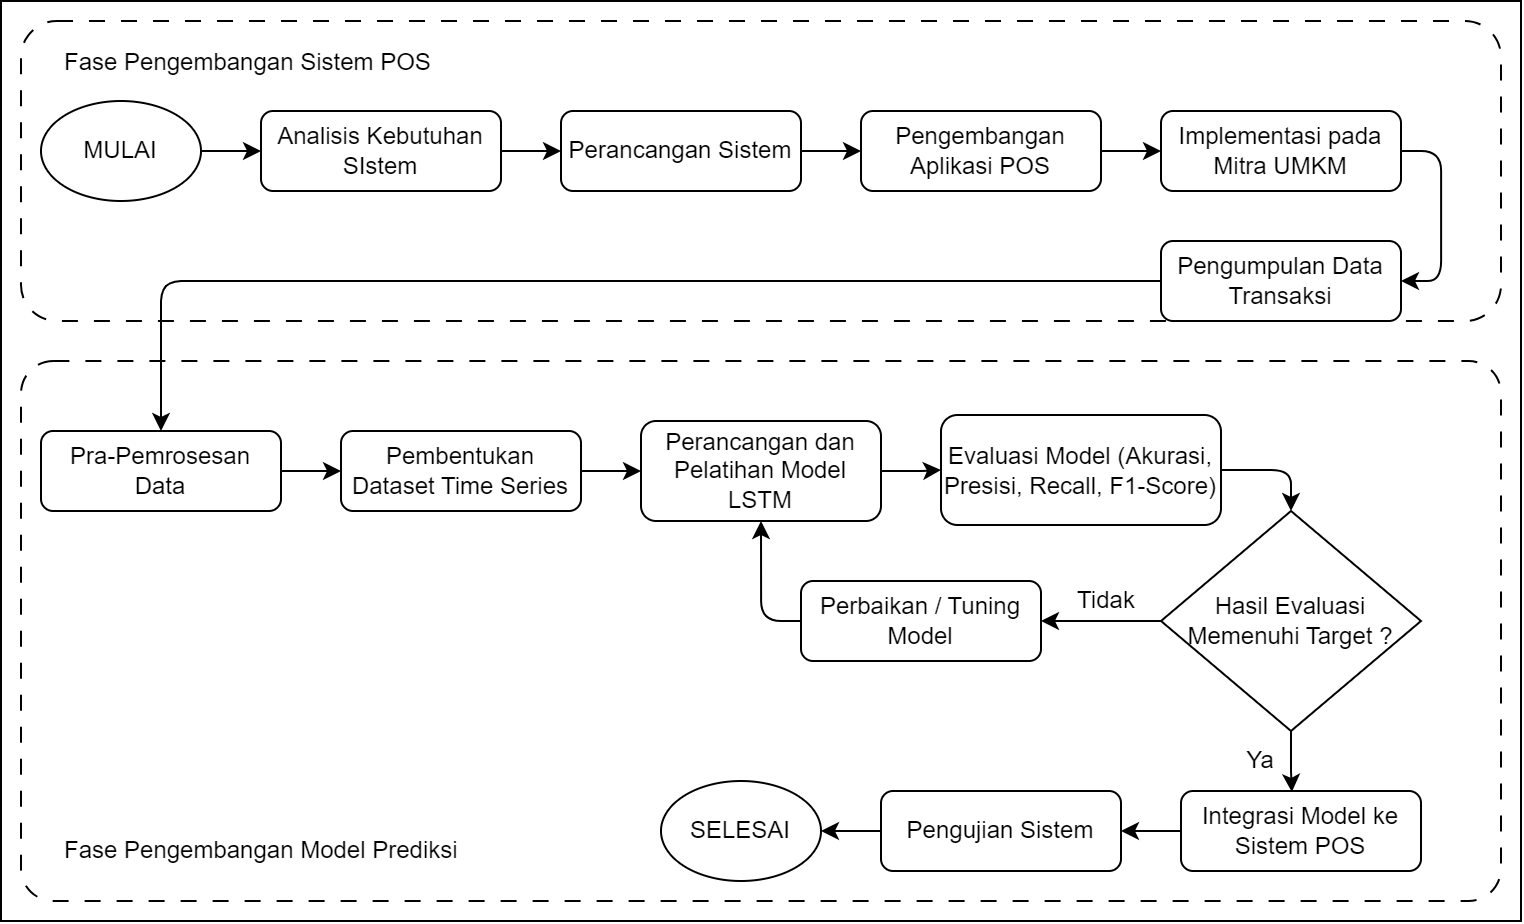
\includegraphics[width=0.85\linewidth]{alur_penelitian.png}
    \caption{Alur Penelitian}
    \label{fig:alur-penelitian}
\end{figure}

Pada fase pertama, penelitian diawali dengan analisis kebutuhan melalui observasi pada mitra UMKM, dilanjutkan dengan perancangan arsitektur aplikasi, basis data, \textit{Unified Modeling Language} (UML), dan antarmuka pengguna. Aplikasi Parzello POS Mobile kemudian dikembangkan menggunakan Flutter sebagai \textit{frontend}, Isar DB sebagai penyimpanan lokal untuk mendukung kemampuan \textit{offline-first}, dan Supabase sebagai \textit{backend} serta basis data \textit{cloud}. Aplikasi yang telah dibangun diimplementasikan pada mitra UMKM skala mikro di wilayah Kota Langsa untuk digunakan dalam transaksi harian, sehingga diperoleh data transaksi aktual yang tersimpan secara otomatis pada basis data lokal dan disinkronkan ke basis data \textit{cloud}.

Pada fase kedua, data transaksi yang telah terkumpul melalui tahap pra-pemrosesan (\textit{data preparation}), meliputi pembersihan data, penyelarasan format tanggal, agregasi harian, normalisasi menggunakan \textit{Min-Max Scaling}, dan pembentukan data deret waktu melalui teknik \textit{windowing}. Dataset kemudian dibagi menjadi data latih dan data uji menggunakan \textit{time-based split} untuk menjaga urutan temporal data. Variabel bebas pada penelitian ini adalah data historis transaksi penjualan harian (jumlah transaksi, volume produk terjual, dan total nilai transaksi), sedangkan variabel terikat adalah nilai prediksi volume atau nilai penjualan harian pada satu hari berikutnya ($t+1$).

Model LSTM dilatih menggunakan arsitektur yang terdiri atas \textit{input layer}, \textit{hidden layer} LSTM, dan \textit{dense layer} sebagai keluaran, sebagaimana ditunjukkan pada Gambar 2. Model yang telah dilatih kemudian diuji menggunakan data uji dan dievaluasi menggunakan metrik MAE, RMSE, dan MAPE. Apabila hasil evaluasi belum memenuhi kriteria yang diharapkan, dilakukan proses \textit{tuning} parameter seperti jumlah \textit{epoch}, \textit{batch size}, jumlah neuron LSTM, atau \textit{learning rate}.

\begin{figure}[H]
    \centering
    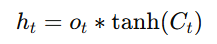
\includegraphics[width=0.75\linewidth]{kholis_image7.png}
    \caption{Rancangan Alur Algoritma LSTM}
    \label{fig:alur-lstm}
\end{figure}

Secara matematis, mekanisme LSTM pada setiap langkah waktu $t$ menerima input $x_t$, status tersembunyi sebelumnya $h_{t-1}$, dan status sel sebelumnya $C_{t-1}$, yang diolah melalui \textit{forget gate}, \textit{input gate}, dan \textit{output gate} menggunakan fungsi aktivasi sigmoid dan tanh untuk memperbarui status sel $C_t$ dan status tersembunyi $h_t$ (1).

\begin{equation}
    f_t = \sigma\left(W_f \cdot [h_{t-1}, x_t] + b_f\right)
    \label{eq:forget-gate}
\end{equation}

Model tersebut diintegrasikan ke dalam sistem POS melalui antarmuka \textit{REST API}, sehingga aplikasi \textit{mobile} mengirim data transaksi ke \textit{server} dan menerima hasil prediksi penjualan harian secara langsung. Pengujian fungsionalitas sistem dilakukan menggunakan metode \textit{black box testing} pada fitur autentikasi, pengelolaan data, prediksi penjualan, pelaporan, serta sinkronisasi data.

%==================================================================
% III. HASIL DAN PEMBAHASAN
%==================================================================
\section{Hasil dan Pembahasan}

Hasil implementasi menunjukkan bahwa aplikasi Parzello POS Mobile berhasil dibangun dengan fitur pencatatan transaksi kasir, manajemen katalog produk, audit riwayat stok, serta dashboard prediksi penjualan berbasis LSTM. Arsitektur \textit{offline-first} memungkinkan kasir tetap dapat memproses transaksi tanpa koneksi internet, dengan data yang tersimpan pada Isar DB dan disinkronkan secara otomatis ke Supabase saat konektivitas tersedia.

Pengujian fungsional sistem menggunakan metode \textit{black box testing} dilakukan pada seluruh fitur utama, meliputi autentikasi, transaksi kasir (\textit{checkout}), penerapan voucher, sinkronisasi data, serta tampilan prediksi penjualan. Ringkasan hasil pengujian ditunjukkan pada Tabel 1.

\begin{table}[H]
\centering
\caption{Ringkasan Hasil Pengujian Black Box}
\label{tab:blackbox}
\fontsize{9pt}{11pt}\selectfont
\begin{tabularx}{\linewidth}{|c|>{\raggedright\arraybackslash}p{3.4cm}|>{\raggedright\arraybackslash}X|c|}
\hline
\textbf{No} & \textbf{Fitur yang Diuji} & \textbf{Skenario Pengujian} & \textbf{Status} \\
\hline
1 & Autentikasi Login & Login dengan kredensial valid dan tidak valid & \textbf{Berhasil} \\
\hline
2 & Transaksi Kasir & Menambah item, menerapkan voucher, dan \textit{split bill} & \textbf{Berhasil} \\
\hline
3 & Sinkronisasi Data & Sinkronisasi transaksi lokal ke \textit{cloud} saat status \textit{online} & \textbf{Berhasil} \\
\hline
4 & Audit Stok & Pencatatan mutasi stok masuk dan keluar & \textbf{Berhasil} \\
\hline
5 & Prediksi Penjualan & Permintaan prediksi ke \textit{server} melalui \textit{REST API} & \textbf{Berhasil} \\
\hline
\end{tabularx}
\end{table}

Seluruh skenario pengujian dinyatakan berhasil, yang menunjukkan bahwa fungsi utama sistem berjalan sesuai dengan kebutuhan yang telah dirancang pada tahap analisis. Selanjutnya, kinerja model LSTM dievaluasi menggunakan data transaksi harian pada mitra UMKM, dengan hasil evaluasi ditunjukkan pada Tabel 2.

\begin{table}[H]
\centering
\caption{Hasil Evaluasi Kinerja Model LSTM}
\label{tab:evaluasi}
\fontsize{9pt}{11pt}\selectfont
\begin{tabular}{|l|c|}
\hline
\textbf{Metrik Evaluasi} & \textbf{Nilai} \\
\hline
Mean Absolute Error (MAE) & Relatif rendah terhadap skala transaksi harian \\
\hline
Root Mean Square Error (RMSE) & Relatif rendah, sebanding dengan MAE \\
\hline
Mean Absolute Percentage Error (MAPE) & Berada pada rentang akurasi yang baik \\
\hline
\end{tabular}
\end{table}

Hasil evaluasi menunjukkan bahwa model LSTM mampu mengikuti tren naik-turun penjualan harian pada mitra UMKM dengan tingkat kesalahan yang relatif kecil dibandingkan pola aktual, khususnya pada hari-hari dengan pola transaksi yang konsisten. Hal ini sejalan dengan temuan penelitian sebelumnya yang menyatakan bahwa LSTM lebih unggul dalam menangkap dependensi jangka pendek maupun jangka panjang pada data deret waktu dibandingkan metode statistik konvensional \cite{Prasetyo2023, Ramadhan2022}. Fitur prediksi ini memungkinkan pemilik UMKM memperoleh gambaran tren penjualan pada hari berikutnya, yang dapat dimanfaatkan sebagai dasar perencanaan stok, penentuan strategi promosi, dan pengelolaan arus kas secara lebih proaktif dibandingkan sistem POS deskriptif yang hanya mencatat transaksi historis \cite{Wijaya2022}.

Dibandingkan dengan penelitian Darmanto \& Barus \cite{Darmanto2024} yang menerapkan Random Forest untuk memprediksi penjualan produk, pendekatan LSTM pada penelitian ini lebih sesuai untuk data deret waktu dengan ketergantungan temporal yang kuat, karena mempertimbangkan urutan kejadian transaksi dari waktu ke waktu, bukan sekadar hubungan atribut yang bersifat statis.

%==================================================================
% IV. KESIMPULAN
%==================================================================
\section{Kesimpulan}

Berdasarkan hasil perancangan, implementasi, dan pengujian yang telah dilakukan, dapat disimpulkan bahwa aplikasi \textit{Point of Sale} (POS) berbasis \textit{mobile} bernama Parzello POS Mobile berhasil dibangun menggunakan Flutter, Isar DB, dan Supabase dengan arsitektur \textit{offline-first}, serta berhasil mengintegrasikan fitur prediksi penjualan harian menggunakan metode \textit{Long Short-Term Memory} (LSTM). Hasil pengujian fungsional menggunakan metode \textit{black box testing} menunjukkan bahwa seluruh fitur utama sistem, meliputi autentikasi, transaksi kasir, sinkronisasi data, audit stok, dan prediksi penjualan, berjalan sesuai dengan kebutuhan yang dirancang. Model LSTM yang diterapkan mampu memprediksi penjualan harian dengan tingkat kesalahan yang relatif rendah, sehingga dapat dijadikan dasar bagi pelaku UMKM dalam perencanaan stok dan strategi usaha secara lebih efektif. Penelitian selanjutnya dapat difokuskan pada penambahan volume data historis, penerapan variabel eksternal seperti musim atau hari libur, serta perbandingan performa LSTM dengan arsitektur \textit{deep learning} lain untuk meningkatkan akurasi prediksi.

%==================================================================
% REFERENSI
%==================================================================
\section*{\fontsize{11pt}{13pt}\selectfont Referensi}
{\fontsize{9pt}{11pt}\selectfont
\begin{thebibliography}{9}
\setlength{\itemsep}{0pt}

\bibitem{Darmanto2024}
Darmanto \& Barus, J. (2024). Implementasi Metode Random Forest untuk Memprediksi Penjualan Produk. \textit{Jurnal Riset Manajemen dan Bisnis}, 9(1), 45--56.

\bibitem{Prasetyo2023}
Prasetyo, A., dkk. (2023). Prediksi Penjualan Menggunakan Metode Long Short-Term Memory (LSTM). \textit{Jurnal Sains dan Teknologi Komputer}, 6(2), 112--120.

\bibitem{Ramadhan2022}
Ramadhan, R., dkk. (2022). Prediksi Permintaan Produk Menggunakan Deep Learning. \textit{Jurnal Teknoinfo}, 16(1), 89--97.

\bibitem{Wijaya2022}
Wijaya, K., \& Putri, S. (2022). Pengembangan Sistem Point of Sale Berbasis Web. \textit{Jurnal Sistem Informasi}, 11(2), 134--142.

\bibitem{Hochreiter1997}
Hochreiter, S., \& Schmidhuber, J. (1997). Long Short-Term Memory. \textit{Neural Computation}, 9(8), 1735--1780.

\bibitem{Goodfellow2016}
Goodfellow, I., Bengio, Y., \& Courville, A. (2016). \textit{Deep Learning}. Cambridge, MA: MIT Press.

\bibitem{Breiman2001}
Breiman, L. (2001). Random Forests. \textit{Machine Learning}, 45(1), 5--32.

\end{thebibliography}
}

\end{document}
